\exercise

Given the string set $S$ = \{ \texttt{bacco}, \texttt{bit}, \texttt{car},
\texttt{cat}, \texttt{costly}, \texttt{bach}, \texttt{bitly}, \texttt{coat},
\texttt{baccus}, \texttt{bus}, \texttt{cod}, \texttt{cost} \}, show the 2-level
indexing of $S$ for an internal memory able to store 3 string and thus
illustrate the execution of the query $P = \texttt{baccus}$, countin how many
I/O are executed.

\solution

First, we sort the strings on the disk, obtaining $S_{sort}$ = \{
\texttt{bacco}, \texttt{baccus}, \texttt{bach}, \texttt{bit}, \texttt{bitly},
\texttt{bus},\texttt{car}, \texttt{cat}, \texttt{coat}, \texttt{cod},
\texttt{cost}, \texttt{costly} \}. Then, since we can store only 3 strings in
memory, we divide the set in 3 (balanced) parts (buckets) and we use the first
string of each bucket as key:
%
\begin{align*}
  B_1 &= \{ \underline{\texttt{bacco}}, \texttt{baccus}, \texttt{bach},
  \texttt{bit} \} \\
  B_2 &= \{ \underline{\texttt{bitly}}, \texttt{bus},\texttt{car}, \texttt{cat}
  \} \\
  B_3 &= \{ \underline{\texttt{coat}}, \texttt{cod}, \texttt{cost},
  \texttt{costly} \}
\end{align*}
%
Notice that the keys are stored in the index in internal memory, so there is no
need to store them also in the buckets in the external memory. We build the
index as a trie, as in the following picture:
%
\begin{figure}[H]
  \centering
  \tikzstyle{level 1}=[level distance=2cm, sibling distance=3cm]
  \tikzstyle{level 2}=[level distance=2cm, sibling distance=2cm]
  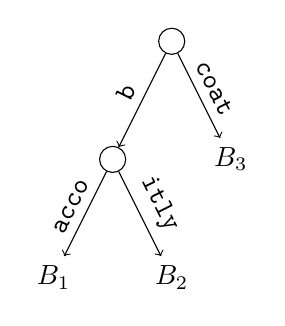
\begin{tikzpicture}[grow=down, sloped]
  \node[draw,fill=white, circle] {}
      child {
          node[draw,fill=white, circle] {}
              child {
                  node[draw=none,fill=none] {$B_1$}
                  edge from parent[->]
                  node[above] {\tt acco}
              }
              child {
                  node[draw=none,fill=none] {$B_2$}
                  edge from parent[->]
                  node[above] {\tt itly}
              }
              edge from parent[->]
              node[above] {\tt b}
      }
      child {
          node[draw=none,fill=none] {$B_3$}
          edge from parent[->]
          node[above] {\tt coat}
      };
  \end{tikzpicture}
\end{figure}
%
The buckets are stored using front coding:
%
\begin{longtable}{l}
  \begin{tabular}{rccc}
    \null & $\null_\texttt{baccus}$ & $\null_\texttt{bach}$ &
    $\null_\texttt{bit}$ \\
    $B_1 \rightarrow$ (\texttt{bacco}) & $\langle 6, 4, \texttt{us} \rangle$ &
    $\langle 4, 3, \texttt{h} \rangle$ & $\langle 3, 1, \texttt{it} \rangle$ \\
  \end{tabular} \\
  \begin{tabular}{rccc}
    \null & $\null_\texttt{bus}$ & $\null_\texttt{car}$ & $\null_\texttt{cat}$\\
    $B_2 \rightarrow$ (\texttt{bitly}) & $\langle 3, 1, \texttt{us} \rangle$ &
    $\langle 3, 0, \texttt{car} \rangle$ & $\langle 3, 2, \texttt{t} \rangle$ \\
  \end{tabular} \\
  \begin{tabular}{rccc}
    \null & $\null_\texttt{cod}$ & $\null_\texttt{cost}$ &
    $\null_\texttt{costly}$ \\
    $B_3 \rightarrow$ (\texttt{coat}) & $\langle 3, 2, \texttt{d} \rangle$ &
    $\langle 4, 2, \texttt{st} \rangle$ & $\langle 6, 4, \texttt{ly} \rangle$ \\
  \end{tabular}
\end{longtable}
%
Notice that \texttt{bit} and \texttt{bitly} are very similar, so it would be
great to put them in the same bucket, increasing their compression.

To compute the query we make a lexicographic search (\emph{not an exact search})
for the string \texttt{baccus}. We visit the trie, and we discover that the
string, if it exists, is between \texttt{bacco} and \texttt{bitly}, so in $B_1$.
We scan it and find it in the first block, so only an I/O operation is needed.
